\documentclass{experimento}

    % UNITS
\usepackage{siunitx}
\sisetup{per-mode=symbol}

    % GRAPHICS
\usepackage{tikz}
\usepackage{pgfplots}
\pgfplotsset{width=7cm,compat=1.3}

\begin{document}

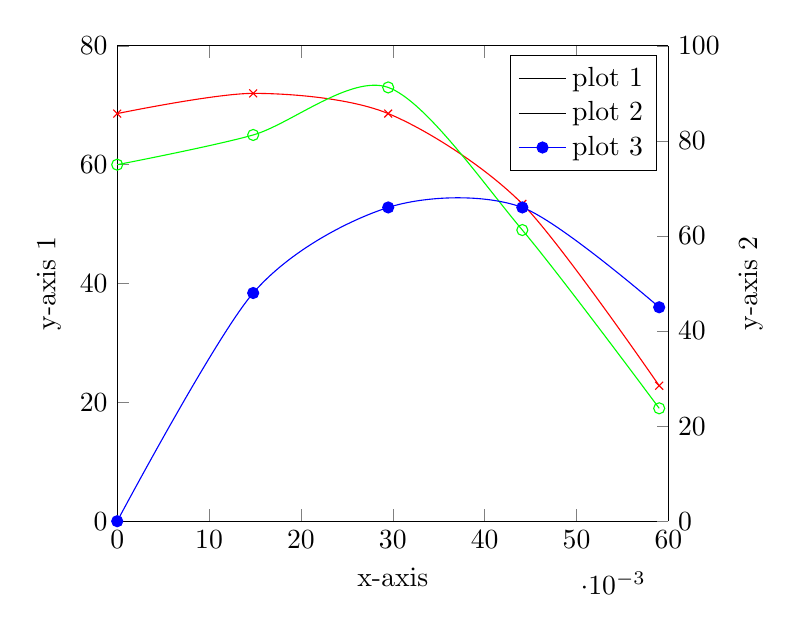
\begin{tikzpicture}
\pgfplotsset{
    scale only axis,
    scaled x ticks=base 10:3,
    xmin=0, xmax=0.06
}

\begin{axis}[
  axis y line*=left,
  ymin=0, ymax=80,
  xlabel=x-axis,
  ylabel=y-axis 1,
]
\addplot[smooth,mark=x,red]
  coordinates{
    (0,68.6)
    (0.0148,72)
    (0.0295,68.6)
    (0.0441,53.4)
    (0.059,22.8)
}; \label{plot_one}

\addplot[smooth,mark=o,green]
  coordinates{
    (0,60)
    (0.0148,65)
    (0.0295,73)
    (0.0441,49)
    (0.059,19)
}; \label{plot_two}

\end{axis}

\begin{axis}[
  axis y line*=right,
  axis x line=none,
  ymin=0, ymax=100,
  ylabel=y-axis 2
]
\addlegendimage{/pgfplots/refstyle=plot_one}\addlegendentry{plot 1}
\addlegendimage{/pgfplots/refstyle=plot_two}\addlegendentry{plot 2}
\addplot[smooth,mark=*,blue]
  coordinates{
    (0,0)
    (0.0148,48)
    (0.0295,66)
    (0.0441,66)
    (0.059,45.0)
}; \addlegendentry{plot 3}
\end{axis}

\end{tikzpicture}
\end{document}